\documentclass{article}
\usepackage{amsfonts} % For open face letters
\usepackage{amsmath} % For align*
\usepackage{float} % For the [H] option on figures
\usepackage{graphicx} % For images
\usepackage{siunitx} % For units
\graphicspath{{./images/}}

\renewcommand{\vec}[1]{\boldsymbol{\mathbf{#1}}}
\newcommand{\dvec}[1]{\dot{\vec{#1}}}
\newcommand{\ddvec}[1]{\ddot{\vec{#1}}}
\newcommand{\uvec}[1]{\hat{\vec{#1}}}

\newcommand{\ke}{\frac{1}{4 \pi \epsilon_0}}

\def\rcurs{{\mbox{$\resizebox{.09in}{.08in}{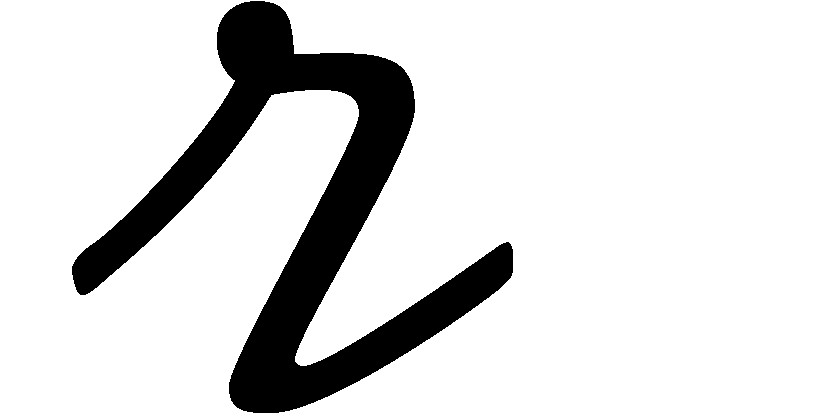
\includegraphics[trim= 1em 0 14em 0,clip]{ScriptR}}$}}}
\def\brcurs{{\mbox{$\resizebox{.09in}{.08in}{
\includegraphics[trim= 1em 0 14em 0,clip]{BoldR}}$}}}
\def\hrcurs{{\mbox{$\hat \brcurs$}}}

\title{Introduction to Electrodynamics by David J. Griffiths Notes}
\author{Chris Doble}
\date{December 2023}

\begin{document}

\maketitle

\tableofcontents

\section{Vector Algebra}

\setcounter{subsection}{5}
\subsection{The Theory of Vector Fields}

\subsubsection{The Helmholtz Theorem}

\begin{itemize}
  \item The \textbf{Helmholtz theorem} states that a vector field $\vec{F}$ is uniquely determined if you're given its divergence $\nabla \cdot \vec{F}$, curl $\nabla \times \vec{F}$, and sufficient boundary conditions.
\end{itemize}

\subsubsection{Potentials}

\begin{itemize}
  \item If the curl of a vector field vanishes everywhere, then it can be expressed as the gradient of a \textbf{scalar potential} \[\nabla \times \vec{F} = \vec{0} \Leftrightarrow \vec{F} = -\nabla V.\]

  \item If the divergence of a vector field vanishes everywhere, then it can be expressed as the curl of a \textbf{vector potential} \[\nabla \cdot \vec{F} = 0 \Leftrightarrow \vec{F} = \nabla \times \vec{A}.\]
\end{itemize}

\section{Electrostatics}

\subsection{The Electric Field}

\setcounter{subsubsection}{1}
\subsubsection{Coulomb's Law}

\begin{itemize}
  \item \textbf{Couloumb's law} gives the force between two point charges $q$ and $Q$ \[\vec{F} = \frac{1}{4 \pi \epsilon_0} \frac{q Q}{\rcurs} \hrcurs\] where \[\epsilon_0 = \qty{8.85e-12}{C^2/(N.m^2)}\] is the \textbf{permittivity of free space} and $\brcurs$ is the separation vector between the two charges.
\end{itemize}

\subsubsection{The Electric Field}

\begin{itemize}
  \item The \textbf{electric field} $\vec{E}$ is a vector field that varies from point to point and gives the force per unit charge that would be exerted on a test charge if placed at a particular point.

  \item For a collection of $n$ source charges $q_i$ at displacements $\brcurs_i$ from a test charge, the electric field is \[\vec{E} = \frac{1}{4 \pi \epsilon_0} \sum_{i = 1}^n \frac{q_i}{\rcurs_i^2} \hrcurs.\]
\end{itemize}

\subsubsection{Continuous Charge Distributions}

\begin{itemize}
  \item Couloumb's law for a continuous charge distribution is \[\vec{E} = \ke \int \frac{1}{\rcurs^2} \hrcurs \,d q.\]
\end{itemize}

\subsection{Divergence and Curl of Electrostatic Fields}

\subsubsection{Field Lines, Flux, and Gauss's Law}

\begin{itemize}
  \item \textbf{Gauss's law} states that the electric field flux through a closed surface is proportional to the amount of charge within that surface \[\oint \vec{E} \cdot d \vec{a} = \frac{1}{\epsilon_0} Q_\text{enc}\] or \[\nabla \cdot \vec{E} = \frac{1}{\epsilon_0} \rho.\]
\end{itemize}

\setcounter{subsubsection}{3}
\subsubsection{The Curl of E}

\begin{itemize}
  \item The curl of an electric field is $\vec{0}$ \[\nabla \times \vec{E} = \vec{0}.\]
\end{itemize}

\subsection{Electric Potential}

\subsubsection{Introduction to Potential}

\begin{itemize}
  \item The \textbf{electric potential} at a point $\vec{r}$ is defined as \[V(\vec{r}) = -\int_\mathcal{O}^{\vec{r}} \vec{E} \cdot d \vec{l}\] where $\mathcal{O}$ is an agreed origin.

  \item The potential difference between two points $\vec{a}$ and $\vec{b}$ is \[V(\vec{b}) - V(\vec{a}) = -\int_{\vec{a}}^{\vec{b}} \vec{E} \cdot d \vec{l}.\]

  \item The electric field and potential are also related by the equation \[\vec{E} = -\nabla V.\]
\end{itemize}

\subsubsection{Comments on Potential}

\begin{itemize}
  \item The choice of origin $\mathcal{O}$ in the definiton of vector potential only affects the absolute potential values, not potential differences. Typically it is chosen to be ``at infinity'' unless the charge distribution itself extends to infinity.

  \item Electric potential obeys the superposition principle.

  \item The units of electric potential is $\unit{N.m/C} = \unit{J/C} = \unit{V}$.
\end{itemize}

\subsubsection{Poisson's Equation and Laplace's Equation}

\begin{itemize}
  \item If \[\nabla \cdot \vec{E} = \frac{\rho}{\epsilon_0}\] and \[\vec{E} = -\nabla V\] then \begin{align*}
          \nabla \cdot (-\nabla V) & = \frac{\rho}{\epsilon_0}   \\
          \nabla^2 V               & = -\frac{\rho}{\epsilon_0}.
        \end{align*} This is known as \textbf{Poisson's equation}. In regions where $\rho = 0$ it reduces to \textbf{Laplace's equation} \[\nabla^2 V = 0.\]
\end{itemize}

\subsubsection{The Potential of a Localized Charge Distribution}

\begin{itemize}
  \item The potential of a continuous charge distribution is \[V(\vec{r}) = \ke \int \frac{\rho(\vec{r}')}{\rcurs} \,d \tau'\] where the reference is point is set to infinity.
\end{itemize}

\subsubsection{Boundary Conditions}

\begin{figure}[H]
  \centering
  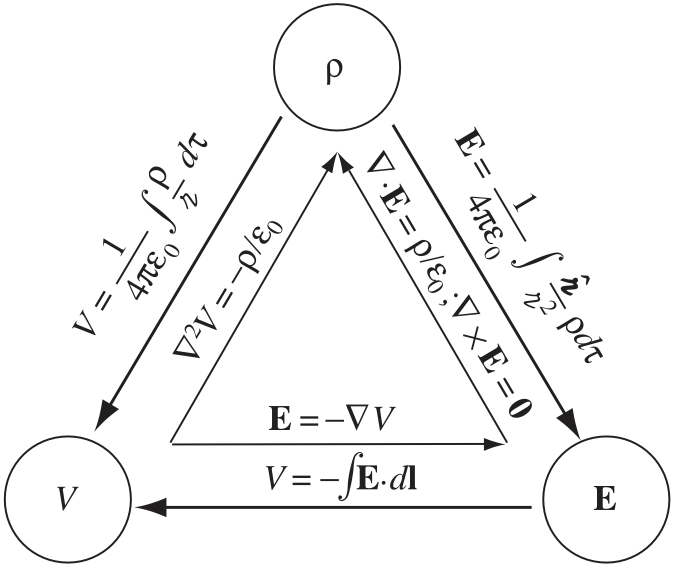
\includegraphics[scale=0.5]{electrostatic-relations}
\end{figure}

\begin{itemize}
  \item The normal component of the electric field is discontinuous by an amount $\sigma / \epsilon_0$ at any boundary, i.e. \[E_\text{above} - E_\text{below} = \frac{\sigma}{\epsilon_0}.\]

  \item The tangential component of the electric field is always continuous at any boundary.

  \item The electric potential is always continuous at any boundary, however because $\vec{E} = -\nabla V$, the gradient of the electric potential inherits the discontinuity at boundaries with surface charge, i.e. \[\nabla V_\text{above} - \nabla V_\text{below} = -\frac{\sigma}{\epsilon_0} \uvec{n}\] or \[\frac{\partial V_\text{above}}{\partial n} - \frac{\partial V_\text{below}}{\partial n} = -\frac{\sigma}{\epsilon_0}\] where \[\frac{\partial V}{\partial n} = \nabla V \cdot \uvec{n}.\]
\end{itemize}

\subsection{Work and Energy in Electrostatics}

\subsubsection{The Work It Takes to Move a Charge}

\begin{itemize}
  \item The work required to move a charge $Q$ from infinity to a point $\vec{r}$ is \[W = Q [V(\vec{r}) - V(\infty)] = Q V(\vec{r}).\] In that sense, the electric potential is the energy per unit charge required to assemble a system of point charges.
\end{itemize}

\subsubsection{The Energy of a Point Charge Distribution}

\begin{itemize}
  \item If you bring a first charge in from infinity you do no work because there are no other charges. If you bring a second charge in from inifnity you do work against the electric field of the first charge. The third does work against the first and second, and so on. Thus the total work required to assemble a collection of charges is \begin{align*}
          W & = \ke \left( \frac{q_1 q_2}{\rcurs_{1 2}} + \frac{q_1 q_3}{\rcurs_{1 3}} + \ldots + \frac{q_1 q_n}{\rcurs{1 n}} + \frac{q_2 q_3}{\rcurs_{2 3}} + \ldots \right) \\
            & = \ke \sum_{i = 1}^n \sum_{j > i}^n \frac{q_i q_j}{\rcurs_{i j}}
        \end{align*} or if we count each pair of charges twice and divide by two \[W = \frac{1}{8 \pi \epsilon_0} \sum_{i = 1}^n \sum_{j \ne i}^n \frac{q_i q_j}{\rcurs_{i j}}.\] If we pull $q_i$ out the front we get \[W = \frac{1}{2} \sum_{i = 1}^n q_i \left( \sum_{j \ne i}^n \ke \frac{q_j}{\rcurs{i j}} \right) = \frac{1}{2} \sum_{i = 1}^n q_i V(\vec{r}_i).\]
\end{itemize}

\subsubsection{The Energy of a Continuous Charge Distribution}

\begin{itemize}
  \item For a volume charge density $\rho$ the work to assemble a continuous charge distribution is \[W = \frac{1}{2} \int \rho V \,d \tau\] or equivalently \[W = \frac{\epsilon_0}{2} \int E^2 \,d \tau\] where the integral is taken over all space.
\end{itemize}

\subsubsection{Comments on Electrostatic Energy}

\begin{itemize}
  \item The energy of an electrostatic field does not obey the superposition principle.
\end{itemize}

\subsection{Conductors}

\subsubsection{Basic Properties}

\begin{itemize}
  \item $\vec{E} = \vec{0}$ inside a conductor because any net electric field causes charges to move, resulting in an induced charge that cancels the electric field.

  \item $\rho = 0$ inside a conductor. By Gauss's law, if $\vec{E} = \vec{0}$ then $\rho$ must also be $0$.

  \item Any net charge resides on the surface of a conductor.

  \item A conductor is an equipotential, i.e. the electric potential is the same everywhere in the conductor.

  \item $\vec{E}$ is perpendicular to the surface of the conductor. If there was a tangential component, charge would move to cancel it.
\end{itemize}

\subsubsection{Induced Charges}

\begin{itemize}
  \item If you hold a charge near an uncharged conductor, the two will attract one another. This is because the external charge causes charges within the conductor to move in order to cancel its magnetic field — like charges are repelled and unlike charges are attracted. This results in unlike charges being closer to the external charge and like charges being further away, resulting in a net attraction.

  \item If you place a charge in a cavity within a conductor, a charge will be induced on the inner surface of the conductor to negate the charge's field within the conductor. If you apply Gauss's law to a Gassian surface that contains the inner charge and inner surface but not the outer surface, the enclosed charge must be $0$. Thus there must be an induced charge of $q$ on the outer surface which communicates the presence of the inner charge to the outside world.

  \item If a cavity within a conductor contains no charge, $\vec{E} = \vec{0}$ within the cavity.
\end{itemize}

\subsubsection{Surface Charge and Force on a Conductor}

\begin{itemize}
  \item Because the field inside a conductor is zero, the boundary condition $E_\text{above} - E_\text{below} = \sigma / \epsilon_0$ requires that the field immediately outside the conductor is \[\vec{E} = \frac{\sigma}{\epsilon_0} \uvec{n}.\] In terms of potential this is \[\sigma = -\epsilon_0 \frac{\partial V}{\partial n}.\]

  \item In the presence of an electric field, a surface charge will experience a force per unit area \[\vec{f} = \sigma \vec{E}_\text{average} = \frac{1}{2} \sigma (\vec{E}_\text{above} + \vec{E}_\text{below}).\] This applies to any surface charge, however for a conductor $\vec{E}_\text{below} = \vec{0}$ so \[\vec{f} = \frac{1}{2} \sigma \vec{E}_\text{above} = \frac{\sigma^2}{2 \epsilon_0} \uvec{n}.\] Notice that this is independent of the sign of $\sigma$. This results in an outward \textbf{electrostatic pressure} on the surface \[P = \frac{\epsilon_0}{2} E^2\] tending to draw the conductor into the field.
\end{itemize}

\subsubsection{Capacitors}

\begin{itemize}
  \item If you have two conductors and place a charge of $+Q$ on one and $-Q$ on the other, an electric field will be induced between them. By Couloumb's law the electric field is proportional to the charge so doubling the charge doubles the electric field and thus the electric potential. The constant of proportionality between the charge and the potential difference between the condutors is called their \textbf{capacitance} \[C = \frac{Q}{V}\] the unit of which is \textbf{farads} ($\unit{F}$).

  \item The work required to fully charge a capacitor to potential difference $V$ is \[W = \frac{1}{2} C V^2.\]
\end{itemize}

\section{Potentials}

\subsection{Laplace's Equation}

\subsubsection{Introduction}

\begin{itemize}
  \item The primary task of electrostatics is to find the electric field of a stationary charge distribution. In theory this is possible using Couloumb's law, but the integrals are often too difficult. It's often easier to first calculate the potential, but sometimes these too are too difficult. In those cases we can instead try to solve Poisson's equation \[\nabla^2 V = -\frac{\rho}{\epsilon_0}\] or Laplace's equation \[\nabla^2 V = 0.\]
\end{itemize}

\subsubsection{Laplace's Equation in One Dimension}

\begin{itemize}
  \item The solution to Laplace's equation in one dimension \[\frac{d^2 V}{d x^2} = 0\] is \[V = m x + b.\]

  \item Under this solution $V(x)$ is the average of $V(x + a)$ and $V(x - a)$ for any $a$ \[V(x) = \frac{1}{2} [V(x + a) + V(x - a)].\]

  \item Laplace's equation tolerates no maxima or minima between the endpoints.
\end{itemize}

\subsubsection{Laplace's Equation in Two Dimensions}

\begin{itemize}
  \item If you draw a circle of radius $R$ about a point the average value of $V$ on the circle is equal to the value at the centre \[V = \frac{1}{2 \pi R} \oint_\text{circle} V \,d l.\]

  \item $V$ has no maxima or minima — all extrema occur at the boundaries.
\end{itemize}

\subsubsection{Laplace's Equation in Three Dimensions}

\begin{itemize}
  \item The value of $V$ at a point $\vec{r}$ is the average value of $V$ over a spherical surface of radius $R$ centred at $\vec{r}$ \[V(\vec{r}) = \frac{1}{4 \pi R^2} \oint_\text{sphere} V \,d a.\]

  \item $V$ has no maxima or minima — all extrema occur at the boundaries.
\end{itemize}

\subsubsection{Boundary Conditions and Uniqueness Theorems}

\begin{itemize}
  \item The \textbf{first uniqueness theorem} states that the solution to Laplace's equation in some volume $\mathcal{V}$ is uniquely determined if $V$ is specified on the boundary surface $\mathcal{S}$.

  \item A corollary to the first uniqueness theorem is that the potential in a volume $\mathcal{V}$ is uniquely determined if (a) the charge density throughout the region, and (b) the value of $V$ on all boundaries, are specified.
\end{itemize}

\subsubsection{Conductors and the Second Uniqueness Theorem}

\begin{itemize}
  \item The \textbf{second uniqueness theorem} states that in a volume $\mathcal{V}$ surrounded by conductors and containing a specified charge density $\rho$, the electric field is uinquely determined if the total charge on each conductor is given.
\end{itemize}

\subsection{The Method of Images}

\subsubsection{The Classic Image Problem}

\begin{itemize}
  \item By the first uniqueness theorem for solutions to Poisson's equation and Laplace's equation, if we can construct a solution that meets the boundary conditions in the region of interest even if it's different outside the region of interest, that's the solution.

  \item For example, if a point charge $q$ is placed a distance $a$ above an infinite grounded conducting plane it will induce some charge in the plane so it's difficult to calculate the potential. However if we consider an alternate scenario where there's a second point charge $-q$ a distance $a$ below the plane and the plane is removed, the potential is much easier to calculate. Because the boundary conditions in the region $z > 0$ are the same, this potential must be a solution to the original problem.
\end{itemize}

\subsubsection{Induced Surface Charge}

\begin{itemize}
  \item In the problem above, the suface charge induced on the plane can be calculated as \[\sigma = -\epsilon_0 \left. \frac{\partial V}{\partial z} \right|_{z = 0}.\]
\end{itemize}

\subsubsection{Force and Energy}

\begin{itemize}
  \item As potential is the same under the method of images, so is force. Energy however is not the same.
\end{itemize}

\subsubsection{Other Image Problems}

\begin{itemize}
  \item In general, \textbf{the method of images} can be applied when a stationary charge distribution is in the vicinity of an infinite grounding plane by mirroring the charges across the plane and negating their charges.

  \item You can't place image charges in the region where you're trying to calculate the potential — that would change $\rho$ and thus you're solving Poisson's equation with different sources.
\end{itemize}

\subsection{Separation of Variables}

\begin{itemize}
  \item The method of separation of variables can be used to solve Laplace's equation when the potential $V$ or the charge density $\sigma$ is specified on the boundaries of some region.
\end{itemize}

\setcounter{subsubsection}{1}
\subsubsection{Spherical Coordinates}

\begin{itemize}
  \item We assume the problems have \textbf{azimuthal symmetry} so that $V$ is independent of $\phi$.

  \item The solutions to the equation \[\frac{d}{d \theta} \left( \sin \theta \frac{d \Theta}{d \theta} \right) = -l (l + 1) \sin \theta \Theta\] are the \textbf{Legendre polynomials} in the variable $\cos \theta$ \[\Theta(\theta) = P_l(\cos \theta).\] Although there should be two solutions to $\Theta(\theta)$ for each value of $l$, the second set of solutions ``blow up'' at $\theta = 0$ and/or $\theta = \pi$ so can be excluded on physical grounds. If those values of $\theta$ are excluded from the region of interest, then these second solutions must be considered.

  \item Thus, in the case of azimuthal symmetry, the most general separable solution to Laplace's equations is \[V(r, \theta) = \sum_{l = 0}^\infty \left( A r^l + \frac{B}{r^{l + 1}} \right) P_l (\cos \theta).\]
\end{itemize}

\subsection{Multipole Expansion}

\subsubsection{Approximate Potentials at Large Distances}

\begin{itemize}
  \item A \textbf{physical electric dipole} consists of two equal and opposite charges $\pm q$ separated by a distance $d$.

  \item The potential of a dipole at distance $r \gg d$ is \[V(\vec{r}) = \ke \frac{q d \cos \theta}{r^2}\] where $\theta$ is the angle between the line connecting the charges and the line from the centre of the charges to $\vec{r}$.

  \item If we place a pair of dipoles next to each other to make a \textbf{quadrupole}, the potential goes like $1 / r^3$. A pair of quadrupoles back to back makes an \textbf{octopole}, and the potential goes like $1 / r^4$, etc.

  \item The \textbf{multipole expansion} of a charge distribution is an expansion of its potential in terms of powers of $1 / r$ \[V(\vec{r}) = \ke \sum_{n = 0}^\infty \frac{1}{r^{(n + 1)}} \int (r')^n P_n(\cos \alpha) \rho(\vec{r}') \,d \tau'.\]
\end{itemize}

\subsubsection{The Monopole and Dipole Terms}

\begin{itemize}
  \item The dipole term in the multipole expansion is \[V_\text{dip}(\vec{r}) = \ke \frac{1}{r^2} \int r' \cos \alpha \,\rho (\vec{r}') \,d \tau'\] or, since $\cos \alpha$ is the angle between $\vec{r}$ and $\vec{r}'$ \[V_\text{dip}(\vec{r}) = \ke \frac{1}{r^2} \uvec{r} \cdot \int \vec{r}' \rho(\vec{r}') \,d \tau'.\] This integral (which doesn't depend on $\vec{r}$) is called the \textbf{dipole moment} of the distribution \[\vec{p} = \int \vec{r}' \rho(\vec{r}') \,d \tau',\] and the dipole term simplifies to \[V_\text{dip}(\vec{r}) = \ke \frac{\vec{p} \cdot \uvec{r}}{r^2}.\]

  \item The dipole moment for a collection of point charges is \[\vec{p} = \sum^n q_i \vec{r_i}'\] and for physical dipole is \[\vec{p} = q \vec{d}\] where $\vec{d}$ is the vector from the negative charge to the positive charge.

  \item A \textbf{perfect dipole} is one whose potential is described exactly by the dipole term (no higher terms are needed). This occurs when $d \rightarrow 0$ and $q \rightarrow \infty$ while maintaining $q d = p$.

  \item Dipole moments are vectors and add accordingly, e.g. if you have two dipoles $\vec{p}_1$ and $\vec{p}_2$ the total dipole is $\vec{p}_1 + \vec{p}_2$.
\end{itemize}

\subsubsection{Origin of Coordinates in Multipole Expansions}

\begin{itemize}
  \item Because the multipole expansion is a power series in inverse powers of $r$ (the distance to the origin), moving the charge or the origin can affect the expansion. For example, a monopole $q$ at the origin has potential $q / 4 \pi \epsilon_0 r$ — exactly the monopole term in the multipole expansion — but if it is moved a distance $d$ from the origin it gains a dipole moment $q d$.

  \item If the total charge is $0$ the dipole moment doesn't change when you move the distribution or the origin.
\end{itemize}

\subsubsection{The Electric Field of a Dipole}

\begin{itemize}
  \item The electric field of a dipole with $\vec{p}$ pointing in the $z$ direction is \[\vec{E}_\text{dip}(r, \theta) = \ke \frac{p}{r^3} (2 \cos \theta \uvec{r} + \sin \theta \uvec{\theta}).\]
\end{itemize}

\section{Electric Fields in Matter}

\subsection{Polarization}

\subsubsection{Dielectrics}

\begin{itemize}
  \item \textbf{Conductors} have an effectively unlimited number of free electrons — typically one or two per atom aren't bound and can move around.

  \item \textbf{Insulators} or \textbf{dielectrics} have no free electrons — they're all bound to atoms.
\end{itemize}

\subsubsection{Induced Dipoles}

\begin{itemize}
  \item When a neutral atom is placed in an electric field $\vec{E}$ the positive nucleus experiences a force in the direction of $\vec{E}$ and the negative electron cloud experiences a force in the opposite direction to $\vec{E}$. This causes them to separate slightly and the atom is said to be \textbf{polarized}. This also results in a small dipole moment \[\vec{p} = \alpha \vec{E}\] where $\alpha$ is called the \textbf{atomic polarizability}.

  \item Molecules may have different atomic polarizability constants in different directions. In that case, to calculate the resulting dipole moment you must decompose $\vec{E}$ into the relevant directions and multiply them by the relevant constants.

  \item The most general equation for the induced dipole moment of a molecule is \begin{align*}
          p_x & = \alpha_{x x} E_x + \alpha_{x y} E_y + \alpha_{x z} E_z \\
          p_y & = \alpha_{y x} E_x + \alpha_{y y} E_y + \alpha_{y z} E_z \\
          p_z & = \alpha_{z x} E_x + \alpha_{z y} E_y + \alpha_{z z} E_z
        \end{align*} where the set of nine constants $\alpha_{i j}$ constitute the \textbf{polarizability tensor}. The values of the polarizability tensor depend on the axes you choose, but it's always possible to choose axes such that it is a diagonal matrix.
\end{itemize}

\subsubsection{Alignment of Polar Molecules}

\begin{itemize}
  \item Some molecules have a ``built-in'' dipole moment. These are called \textbf{polar molecules}.

  \item A dipole $\vec{p} = q \vec{d}$ in a uniform electric field $\vec{E}$ experiences a torque \[\vec{\tau} = \vec{p} \times \vec{E}.\] This aligns $\vec{p}$ with $\vec{E}$.

  \item A dipole $\vec{p}$ in a nonuniform electric field $\vec{E}$ also experiences a net force \[\vec{F} = \vec{F}_+ + \vec{F}_- = q (\vec{E}_+ - \vec{E}_-) = q (\Delta \vec{E})\] where $\Delta \vec{E}$ is the difference in electric field between the ends of the dipole. If the dipole is very short then \[\vec{F} = (\vec{p} \cdot \nabla) \vec{E}.\]

  \item The energy of an ideal dipole $\vec{p}$ in an electric field $\vec{E}$ is \[U = -\vec{p} \cdot \vec{E}.\]
\end{itemize}

\subsubsection{Polarization}

\begin{itemize}
  \item When an external electric field is applied to a material that consists of neutral atoms or nonpolar molecules, the field will induce in each a small dipole moment pointing in the same direction as the field. If the material consists of polar molecules each will experience a torque aligning it with the field. The net result is that there are many small dipoles pointing in the same direction — the material becomes \textbf{polarized}. A measure of this is \textbf{polarization} $\vec{P}$ which is the dipole moment per unit volume.
\end{itemize}

\subsection{The Field of a Polarized Object}

\subsubsection{Bound Charges}

\begin{itemize}
  \item The potential of a polarized object is equal to that produced by a surface charge density $\sigma_b = \vec{P} \cdot \uvec{n}$ and volume charge density $\rho_b = -\nabla \cdot \vec{P}$, i.e. \[V(\vec{r}) = \ke \oint_\mathcal{S} \frac{\sigma_b}{\rcurs} \,d a' + \ke \int_\mathcal{V} \frac{\rho_b}{\rcurs} \,d \tau'.\] These are called \textbf{bound charges}.
\end{itemize}

\subsection{The Electric Displacement}

\subsubsection{Gauss's Law in the Presence of Dielectrics}

\begin{itemize}
  \item Any charge that is not a result of polarization is called \textbf{free charge} $\rho_f$.

  \item The total charge density is thus \[\rho = \rho_b + \rho_f\] and Gauss's law reads \begin{align*}
          \epsilon_0 \nabla \cdot \vec{E} & = \rho                            \\
                                          & = \rho_b + \rho_f                 \\
                                          & = -\nabla \cdot \vec{P} + \rho_f.
        \end{align*} If we introduce the \textbf{electric displacement} \[\vec{D} = \epsilon_0 \vec{E} + \vec{P}\] then Gauss's law reads \[\nabla \cdot \vec{D} = \rho_f\] or \[\oint \vec{D} \cdot d \vec{a} = Q_{f_\text{enc}}.\]
\end{itemize}

\subsubsection{A Deceptive Parallel}

\begin{itemize}
  \item The curl of $\vec{D}$ is not always zero because \[\nabla \times \vec{D} = \epsilon_0 (\nabla \times \vec{E}) + (\nabla \times \vec{P}) = \nabla \times \vec{P}.\]

  \item As it's curl isn't always zero, there is no scalar potential for $\vec{D}$. If a problem doesn't exhibit the required symmetry to apply Gauss's law for dielectrics we can't fall back on an equivalent of Couloumb's law.
\end{itemize}

\subsubsection{Boundary Conditions}

\begin{itemize}
  \item Like $\vec{E}$, $\vec{D}$ exhibits discontinuities across boundaries \begin{align*}
          D_\text{above}^\perp - D_\text{below}^\perp                     & = \sigma_f                                                         \\
          \vec{D}_\text{above}^\parallel - \vec{D}_\text{below}^\parallel & = \vec{P}_\text{above}^\parallel - \vec{P}_\text{below}^\parallel.
        \end{align*}
\end{itemize}

\subsection{Linear Dielectrics}

\subsubsection{Susceptibility, Permittivity, Dielectric Constant}

\begin{itemize}
  \item A \textbf{linear dielectric} is a material whose polarization is linearly proportional to the applied electric field \[\vec{P} = \epsilon_0 \chi_e \vec{E}\] where $\chi_e$ is a dimensionless proportionality constant called the \textbf{electric susceptibility} of the material and $\vec{E}$ is the total electric field (including that produced by the polarization itself).

  \item The displacement field in linear dielectrics is also proportional to the total electric field \begin{align*}
          \vec{D} & = \epsilon_0 \vec{E} + \vec{P}                   \\
                  & = \epsilon_0 \vec{E} + \epsilon_0 \chi_e \vec{E} \\
                  & = \epsilon_0 (1 + \chi_e) \vec{E}                \\
                  & = \epsilon \vec{E}
        \end{align*} where $\epsilon = \epsilon_0 (1 + \chi_e)$ is the \textbf{permittivity} of the material.

  \item Dividing the permittivity of a material by $\epsilon_0$ gives its \textbf{relative permittivity} or \textbf{dielectric constant} \[\epsilon_r = \frac{\epsilon}{\epsilon_0} = 1 + \chi_e.\]

  \item The line integral of $\vec{P}$ around a closed path that crosses the boundary between two materials may not be zero (e.g. if one material is polarized and the other is not). By Stokes' theorem this means that the curl of $\vec{P}$ is nonzero and thus $\vec{D}$ is nonzero.

  \item In a space filled by a homogeneous linear dielectric then the above doesn't apply and $\nabla \cdot \vec{D} = \rho_f$ and $\nabla \times \vec{D} = \vec{0}$ so $\vec{D}$ can be found from the free charge as if the dielectric weren't there \[\vec{D} = \epsilon_0 \vec{E}_\text{vac}\] and \[\vec{E} = \frac{1}{\epsilon} \vec{D} = \frac{1}{\epsilon_r} \vec{E}_\text{vac}.\]
\end{itemize}

\subsubsection{Boundary Value Problems with Linear Dielectrics}

\begin{itemize}
  \item In a linear dielectric the bound charge density is proportional to the free charge density \[\rho_b = -\nabla \cdot \vec{P} = -\nabla \cdot \left( \epsilon_0 \frac{\chi_e}{\epsilon} \vec{D} \right) = -\left( \frac{\chi_e}{1 + \chi_e} \right) \rho_f.\] This means that, unless charges are embedded in the material, $\rho = 0$, all the charge lies on the surface, and the electric potential within the material obeys Laplace's equation.

  \item Rewriting the boundary conditions for linear dielectrics gives \[\epsilon_\text{above} E_\text{above}^\perp - \epsilon_\text{below} E_\text{below}^\perp = \sigma_f\] or \[\epsilon_\text{above} \frac{\partial V_\text{above}}{\partial n} - \epsilon_\text{below} \frac{\partial V_\text{below}}{\partial n} = -\sigma_f.\]
\end{itemize}

\subsubsection{Energy in Dielectric Systems}

\begin{itemize}
  \item The work required to assemble a system containing linear dielectric material is \[W = \frac{1}{2} \int \vec{D} \cdot \vec{E} \,d \tau.\]
\end{itemize}

\section{Magnetostatics}

\subsection{The Lorentz Force Law}

\setcounter{subsubsection}{1}
\subsubsection{Magnetic Forces}

\begin{itemize}
  \item The force experienced by a charge $Q$ moving at velocity $\vec{v}$ due to a magnetic field $\vec{B}$ is \[\vec{F}_\text{mag} = Q (\vec{v} \times \vec{B}).\]

  \item The \textbf{Lorentz force law} gives the net force on a charge $Q$ moving at velocity $\vec{v}$ in an electric field $\vec{E}$ and a magnetic field $\vec{B}$ \[\vec{F} = Q (\vec{E} + \vec{v} \times \vec{B}).\]

  \item Magnetic forces do no work. They may change the direction in which a particle moves, but can't speed it up or slow it down.
\end{itemize}

\subsubsection{Currents}

\begin{itemize}
  \item The \textbf{current} in a wire the charge per unit time passing a given point.

  \item Current is measured in couloumbs per second or \textbf{amperes} (A).

  \item Current is a vector $\vec{I}$.

  \item The magnetic force on a segment of current-carrying wire is \[\vec{F}_\text{mag} = \int (\vec{v} \times \vec{B}) \,d q = \int (\vec{v} \times \vec{B}) \lambda \,d l = \int (\vec{I} \times \vec{B}) \,d l.\] If $\vec{I}$ and $d \vec{l}$ point in the same direction then \[\vec{F}_\text{mag} = \int I (d \vec{l} \times \vec{B})\] and if $I$ is constant over the wire then \[\vec{F}_\text{mag} = I \int (d \vec{l} \times \vec{B}).\]

  \item When charge flows over a surface we describe it by the \textbf{surface current density} $\vec{K}$. This is the current per unit width.

  \item When charge flows through a volume we describe it by the \textbf{volume current density} $\vec{J}$. This is the current per unit area.

  \item Due to conservation of charge, a net outward flow of current from a volume results in a decrease in the charge density in the volume and a net inflow results in an increase \[\nabla \cdot \vec{J} = -\frac{\partial \rho}{\partial t}.\] This is called the \textbf{continuity equation}.
\end{itemize}

\subsection{The Biot-Savart Law}

\subsubsection{Steady Currents}

\begin{itemize}
  \item Electrostatic is the study of stationary electric charges and their constant electric fields. Magnetostatics is the study of steady electric currents and their constant magnetic fields.

  \item Under magnetostatics the magnitude of a current must be the same all along a wire, otherwise it would pile up somewhere and wouldn't be a steady current. In other words, \[\nabla \cdot \vec{J} = 0.\]
\end{itemize}

\subsubsection{Magnetic Field of a Steady Current}

\begin{itemize}
  \item The magnetic field of a steady current is given by the \textbf{Biot-Savart Law} \[\vec{B} = \frac{\mu_0}{4 \pi} \int \frac{\vec{I} \times \hrcurs}{\rcurs^2} \,d l' = \frac{\mu_0}{4 \pi} I \int \frac{d \vec{l}' \times \hrcurs}{\rcurs^2}\] where $\mu_0 = 4 \pi \times 10^{-7} \,\unit{N/A^2}$ is the \textbf{permeability of free space}.

  \item The units of a magnetic field $\vec{B}$ are \textbf{teslas} (T) where \[\qty{1}{T} = \qty{1}{N/(A.m)}\] or \textbf{gauss} where \[10^4 \,\unit{gauss} = \qty{1}{T}.\]

  \item The magnetic field a distance $s$ from a wire carrying a constant current $I$ is \[\vec{B} = \frac{\mu_0 I}{2 \pi s} \uvec{\phi}.\]

  \item The superposition principle applies to magnetic fields as it does to electric fields.
\end{itemize}

\subsection{The Divergence and Curl of B}

\setcounter{subsubsection}{1}
\subsubsection{The Divergence and Curl of B}

\begin{itemize}
  \item The divergence of a magnetic field is \[\nabla \cdot \vec{B} = 0.\]
\end{itemize}

\subsubsection{Ampère's Law}

\begin{itemize}
  \item \textbf{Ampère's law} gives the curl of a magnetic field \[\nabla \times \vec{B} = \mu_0 \vec{J}\] or in integral form \[\oint \vec{B} \cdot d \vec{l} = \mu_0 I_\text{enc}\] where $I_\text{enc}$ is the amount of current flowing through a surface enclosed by the integral path and the right-hand rule is used to determine what constitutes a positive current (if the fingers of the right hand wrap in the direction of integration then the thumb points in the direction of positive current).
\end{itemize}

\subsection{Magnetic Vector Potential}

\subsubsection{The Vector Potential}

\begin{itemize}
  \item In the same way that $\nabla \times \vec{E} = 0$ permits a scalar electric potential $\vec{E} = -\nabla V$, $\nabla \cdot \vec{B} = 0$ permits a vector magnetic potential \[\vec{B} = \nabla \times \vec{A}.\]

  \item This says nothing about the divergence of $\vec{A}$, however in the same way that you can add any constant to $V$ without affecting $\vec{E}$ you can add the gradient of any scalar to $\vec{A}$ without affecting $\vec{B}$ as the curl of a gradient is $0$. If $\nabla \cdot \vec{A} \ne 0$, adding $\nabla \lambda$ where $\nabla^2 \lambda = -\nabla \cdot \vec{A}$ (which can be solved using the same methods as Laplace or Poisson's equations) results in a divergence of $0$. This means it's always possible to choose $\vec{A}$ such that $\nabla \cdot \vec{A} = 0$.

  \item With the condition that $\nabla \cdot \vec{A} = 0$, Ampère's law becomes \begin{align*}
          \nabla \times \vec{B}                            & = \mu_0 \vec{J}   \\
          \nabla \times (\nabla \times \vec{A})            & = \mu_0 \vec{J}   \\
          \nabla (\nabla \cdot \vec{A}) - \nabla^2 \vec{A} & = \mu_0 \vec{J}   \\
          \nabla^2 \vec{A}                                 & = -\mu_0 \vec{J}.
        \end{align*} This is effectively Possion's equation three times — one for each dimension \begin{align*}
          \nabla^2 A_x & = -\mu_0 J_x  \\
          \nabla^2 A_y & = -\mu_0 J_y  \\
          \nabla^2 A_z & = -\mu_0 J_z.
        \end{align*} Note that in non-cartesian coordinates the unit vectors may also need to be differentiated, meaning the equation can't be split in three like this.

  \item The integral form of Ampère's law using the magnetic potential is \[\oint \vec{A} \cdot d \vec{l} = \Phi\] where $\Phi$ is the flux of $\vec{B}$ through the loop formed by the integral path.

  \item The solutions to Ampère's law using the magnetic potential for line, surface, and volume currents are \begin{align*}
          \vec{A} & = \frac{\mu_0}{4 \pi} \int \frac{\vec{I}}{\rcurs} \,d l'     \\
          \vec{A} & = \frac{\mu_0}{4 \pi} \int \frac{\vec{K}}{\rcurs} \,d a'     \\
          \vec{A} & = \frac{\mu_0}{4 \pi} \int \frac{\vec{J}}{\rcurs} \,d \tau'.
        \end{align*}

  \item In general, the direction of $\vec{A}$ will match the direction of the current.
\end{itemize}

\subsubsection{Boundary Conditions}

\begin{figure}[H]
  \centering
  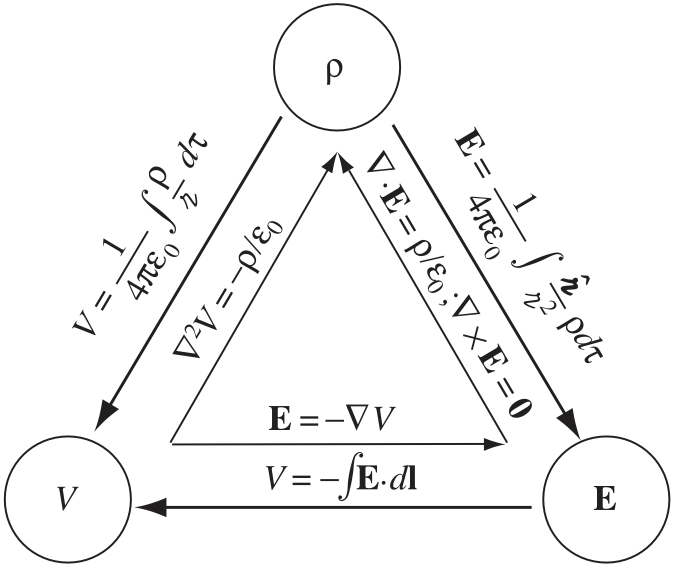
\includegraphics[scale=0.5]{electrostatic-relations}
\end{figure}

\begin{itemize}
  \item Just as the electric field experiences a discontinuity at a surface charge, the magnetic field experiences a discontinuity at a surface current. The continuity of each component can be described as:

        \begin{itemize}
          \item the components perpendicular to the surface are equal \[B_\text{above}^\perp = B_\text{below}^\perp,\]

          \item the components parallel to the surface and parallel to the current are equal, and

          \item the components parallel to the surface and perpendicular to the current experience a discontinuity of $\mu_0 K$.
        \end{itemize}

  \item The above can be summarised as \[\vec{B}_\text{above} - \vec{B}_\text{below} = \mu_0 (\vec{K} \times \uvec{n})\] where $\uvec{n}$ is a unit vector perpendicular to the surface.

  \item Like the electric potential $V$, the magnetic potential $\vec{A}$ is continuous across all boundaries but its derivative is not \[\frac{\partial \vec{A}_\text{above}}{\partial n} - \frac{\partial \vec{A}_\text{below}}{\partial n} = -\mu_0 \vec{K}.\]
\end{itemize}

\subsubsection{Multipole Expansion of the Vector Potential}

\begin{itemize}
  \item The multipole expansion of a localised current distribution is \begin{align*}
          \vec{A}(\vec{r}) & = \frac{\mu_0 I}{4 \pi} \oint \frac{1}{\rcurs} \,d \vec{l}                                                                     \\
                           & = \frac{\mu_0 I}{4 \pi} \sum_{n = 0}^\infty \frac{1}{r^{n + 1}} \oint (r')^n P_n(\cos \alpha) \,d \vec{l}'                     \\
                           & = \frac{\mu_0 I}{4 \pi} \left[ \frac{1}{r} \oint d \vec{l}' + \frac{1}{r^2} \oint r' \cos \alpha \,d \vec{l}' + \cdots \right]
        \end{align*} where $\alpha$ is the angle between $\vec{r}$ and $\vec{r}'$.

  \item In the multipole expansion of the vector potential, the term that goes like $1 / r$ is called the \textbf{monopole} term, $1 / r^2$ the \textbf{dipole} term, etc.

  \item The magnetic monopole term is always zero because \[\oint d \vec{l}' = 0.\] This reflects the fact that magnetic monopoles don't exist.

  \item That being the case, the magnetic dipole term dominates the expansion \[\vec{A}_\text{dip}(\vec{r}) = \frac{\mu_0}{4 \pi} \frac{\vec{m} \times \uvec{r}}{r^2}\] where \[\vec{m} = I \int d \vec{a} = I \vec{a}\] is the \textbf{magnetic dipole moment} and $\vec{a}$ is the vector area of the current loop.

  \item The magnetic field of a dipole can be written as \[\vec{B}_\text{dip}(\vec{r}) = \frac{\mu_0 m}{4 \pi r^3} (2 \cos \theta \uvec{r} + \sin \theta \uvec{\theta})\] or in coordinate-free form \[\vec{B}_\text{dip}(\vec{r}) = \frac{\mu_0}{4 \pi} \frac{1}{r^3} [3 (\vec{m} \cdot \uvec{r}) \uvec{r} - \vec{m}].\]
\end{itemize}

\section{Magnetic Fields in Matter}

\subsection{Magnetization}

\subsubsection{Diamagnets, Paramagnets, Ferromagnets}

\begin{itemize}
  \item In a way, the electrons orbiting an atom form a current, resulting in a magnetic dipole. Thus a material is made up of many small magnetic dipoles. Normally they point in different directions and cancel each other out but if they're aligned the material becomes magnetically polarized or \textbf{magnetized}.

  \item Some materials acquire magnetization parallel to $\vec{B}$ (\textbf{paramagnets}) and some opposite to $\vec{B}$ (\textbf{diamagnets}). A few substances (called \textbf{ferromagnets}) retain their magnetization after the external field is removed.
\end{itemize}

\subsubsection{Torques and Forces on Magnetic Dipoles}

\begin{itemize}
  \item The torque experienced by a localised current distribution in a uniform magnetic field (or the torque experienced by a perfect dipole in a nonuniform magnetic field) is \[\vec{\tau} = \vec{m} \times \vec{B}.\]

  \item The torque above tends to align atomic dipoles with an external magnetic field and explains the phenomenon of paramagnetism.

  \item An infinitesimal loop with dopole moment $\vec{m}$ in a magnetic field $\vec{B}$ experiences a force \[\vec{F} = \nabla (\vec{m} \cdot \vec{B}).\]
\end{itemize}

\subsubsection{Effect of a Magnetic Field on Atomic Orbits}

\begin{itemize}
  \item When subject to an external magnetic field, an electron's orbital speed changes and consequently its magnetic dipole moment. The dipole moment change is opposite to $\vec{B}$ and this the mechanism responsible for \textbf{diamagnetism}.
\end{itemize}

\subsubsection{Magnetisation}

\begin{itemize}
  \item The \textbf{magnetisation} $\vec{M}$ of a material is defined as its magnetic dipole moment per unit volume.
\end{itemize}

\subsection{The Field of a Magnetised Object}

\subsubsection{Bound Currents}

\begin{itemize}
  \item The potential of a magnetised object is the same as would be produced by a volume current \[\vec{J}_b = \nabla \times \vec{M}\] and a surface current \[\vec{K}_b = \vec{M} \times \uvec{n},\] i.e. \[\vec{A}(\vec{r}) = \frac{\mu_0}{4 \pi} \int_\mathcal{V} \frac{\vec{J}_b(\vec{r}')}{\rcurs} \,d \tau' + \frac{\mu_0}{4 \pi} \oint_\mathcal{S} \frac{\vec{K}_b(\vec{r}')}{\rcurs} \,d a'.\] The terms $\vec{J}_b$ and $\vec{K}_b$ are called the bound volume and surface current, respectively.
\end{itemize}

\subsection{The Auxiliary Field H}

\subsubsection{Ampère's Law in Magnetised Materials}

\begin{itemize}
  \item In a magnetised material the total current is \[\vec{J} = \vec{J}_f + \vec{J}_b\] and thus Ampère's law can be written \[\frac{1}{\mu_0} (\nabla \times \vec{B}) = \vec{J} = \vec{J}_f + \vec{J}_b = \vec{J}_f + \nabla \times \vec{M}.\] Moving the curls to one side gives \begin{align*}
          \nabla \times \left( \frac{1}{\mu_0} \vec{B} - \vec{M} \right) & = \vec{J}_f \\
          \nabla \times \vec{H}                                          & = \vec{J}_f
        \end{align*} where $\vec{H} = \vec{B} / \mu_0 - \vec{M}$.

  \item The integral form of Ampère's law in a material is \[\oint \vec{H} \cdot d \vec{l} = I_{f_\text{enc}}.\]
\end{itemize}

\setcounter{subsubsection}{2}
\subsubsection{Boundary Conditions}

\begin{itemize}
  \item The boundary conditions on $\vec{H}$ are \begin{align*}
          H_\text{above}^\perp - H_\text{below}^\perp                     & = -(M_\text{above}^\perp - M_\text{below}^\perp) \\
          \vec{H}_\text{above}^\parallel - \vec{H}_\text{below}^\parallel & = \vec{K}_f \times \uvec{n}
        \end{align*}
\end{itemize}

\end{document}